\chapter{Introduction}

\pagenumbering{arabic}

There is currently a water shortage crisis in South Africa, as well as in other parts of the world, potentially due to global warming. One of the sectors that it affects is agriculture. The water shortage puts added stress on farmers who may already be watering their crops non-uniformly; including the application of fertilizer and pesticides. Even plant disease contributes to the problem.\\

To mitigate such problems, farmers would typically use their expertise in observation from the ground. It can be a time consuming task, especially over areas of a few square kilometres. If static sensor data is used, the readings may be too sparse due to the exponential cost and complexity of multiple static sensors. These sensors require maintenance, post-processing and an estimated interpretation of its data. This does not exclude hand-held readings, which may only be able to point out some areas that need more attention. Perhaps a simpler, large-scale method of observing such changes at once can be used.\\

The human mind is an exceedingly powerful tool to analyse great complexities around the world. Computers may not be as creative, but they boast vast processing power and numerical solving (cite source). Offloading computations and automation better suited for computers from human thought leaves the mind free to do tasks better suited for itself.\\

To observe an area in the digital world, one can observe signals from the electromagnetic spectrum. Although there exists suitable equipment today, it remains yet inaccessible due to the complexity and relatively high cost of equipment. (cite an example) This project looks at a way to bridge this gap somewhat.

\section{Purpose of the project}

The project is conducted to investigate the core elements required to map vegetation via infrared analysis techniques, which can thus potentially determine the impact of human and environmental factors such as diseases, erosion, variances in fertiliser and water application.\\

In order to be deemed successful the project needs to investigate observable parameter(s) beneficial to agriculture within large areas.

\section{Problem Statement}\

To analyse large-scale agricultural areas and produce meaningful data, imagery is typically collected and mathematical algorithms are performed on the data. There are a number of algorithms, with a popular one being the Normalised Differential Vegetation Indice, or NDVI for short. This particular one will be the focus of the project. If successful, it opens up the possibility of investigating other useful indices, perhaps even for the mining industry if this project continues.\\

Cameras will be used to acquire data. Filters will be used to isolate bandwidths required by the vegetation indices.\\

To monitor large areas in a short period of time, one needs height, which can be achieved by the modern invention of flight. In more practical terms, we can use vehicles such as hot air balloons, airstats, planes, helicopters and the like. We can classify these vehicles into manned and unmanned aerial vehicles. Unmanned vehicles have significantly less safety precautions, regulations, cost, and are less subject to wear and tear, meaning more flights (cite).\\

In brief, the idea is to develop a nadir\footnote{Downwards facing} observation platform to map areas from height, to determine observation equipment, to process sampled data and draw conclusions, and to develop control tests to verify / prove conclusions\\

The implementation of autonomous systems can be costly. It also depends on what type of UAV is used. Unmanned aeroplanes  are fast. With enough height, the effects of motion blur tend to zero. On the other hand, they are significantly complex, and although it would be ambitious, it would be impractical for a project such as this. Aerostats\footnote{Lighter than air aircraft that gains its lift through the use of a buoyant gas} and hot air balloons\footnote{Unpowered aerostat which has no means of propulsion and is usually tethered} can stay up for long periods of time, but are impractical due to the limited uses, and difficulty in moving such a vehicle once in the air. Drones on the other hand are inexpensive, and can take accurate and versatile high resolution images, with less risk to the camera equipment than a plane.\\

Thus, a drone is designed and built to demonstrate proof of concept of a more cost effective model compared to solutions that exist in the market today.\\

Various assumptions are made in order to realise the solution of the problem. Besides assumptions regarding the environment in which the system will operate, it will also provide a starting basis for design synthesis. NDVIs are calculated predominantly in the farming sector, the values vary according to the age of the plant, sunlight or clouds will affect the values, and the cameras will be simple to calibrate.

\section{System Overview}

Figure \ref{fig:scenario} illustrates a typical scenario where the system is used.\\

\begin{figure}[H]
\centering
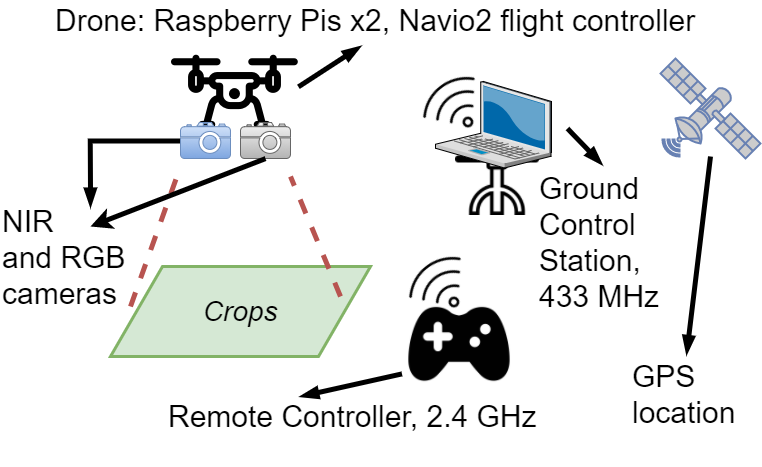
\includegraphics[scale=0.4]{images/drone_ndvi_scenario.png}
\caption{Block diagram system overview}
\label{fig:scenario}
\end{figure}

An implementation process of the system is illustrated in Figure \ref{fig:overview}. These processes will be expanded on and explained in the relevant chapters.

\begin{figure}[H]
\centering
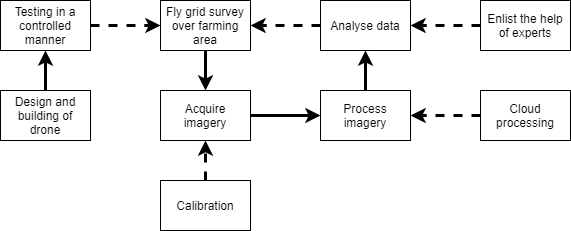
\includegraphics[scale=0.6]{images/thesis_overview.png}
\caption{Block diagram implementation process}
\label{fig:overview}
\end{figure}

Various drones, cameras, filters and processing techniques will be presented, as well as optimal choices depending on available resources.\\

A literature study will be investigated in Chapter 2, with drone design and construction in Chapter 3. Image acquisition and calibration will be handled in Chapter 4, and image processing in Chapter 5. Lastly, system integration and testing will be discussed in Chapter 6.